\documentclass[11pt,a4paper]{article}

\usepackage[utf8]{inputenc}
\usepackage[T1]{fontenc}
\usepackage{lmodern}
\usepackage[margin=2.4cm]{geometry}
\usepackage{amsmath,amssymb}
\usepackage{booktabs}
\usepackage{array}
\usepackage{enumitem}
\usepackage{xcolor}
\usepackage{tikz}
\usetikzlibrary{positioning,calc}
\usepackage[most]{tcolorbox}
\usepackage[htt]{hyphenat}
\usepackage{hyperref}
\usepackage{microtype}
\usepackage{fancyhdr}

\definecolor{accent}{HTML}{1F4E79}
\hypersetup{colorlinks=true, linkcolor=accent, urlcolor=accent}

\newcommand{\code}[1]{\texttt{#1}}
\sloppy
\emergencystretch=3em
\newcolumntype{L}[1]{>{\raggedright\arraybackslash}p{#1}}

\pagestyle{fancy}
\fancyhf{}
\fancyhead[L]{\small\textcolor{gray}{PublicState for Beginners}}
\fancyhead[R]{\small\textcolor{gray}{\code{order\_book}}}
\fancyfoot[C]{\small\thepage}
\renewcommand{\headrulewidth}{0.3pt}

\tcbset{
  boxstyle/.style={enhanced, breakable, colback=#1!6, colframe=#1!70!black,
                   boxrule=0.4pt, arc=2pt, left=8pt, right=8pt, top=5pt, bottom=5pt,
                   fonttitle=\bfseries\small}
}
\newtcolorbox{intuition}{boxstyle=green!50!black, title=In plain words}
\newtcolorbox{example}{boxstyle=orange!90!black, title=Tiny example}
\newtcolorbox{whyuse}{boxstyle=accent, title=Why it is used}

\usepackage{titlesec}
\titleformat{\section}{\Large\bfseries\color{accent}}{\thesection}{0.6em}{}[\vspace{-0.6em}\textcolor{accent!40}{\rule{\linewidth}{0.5pt}}]
\titleformat{\subsection}{\large\bfseries\color{accent!85!black}}{\thesubsection}{0.6em}{}

\title{\textbf{\Huge Understanding \code{PublicState}}\\[8pt]
       \large A gentle, jargon-free guide to the numbers every trader in the simulator can see}
\author{The \code{order\_book} project}
\date{October 2026}

\begin{document}
\maketitle
\thispagestyle{fancy}

\begin{abstract}
\noindent
In the simulator, every participant (noise traders, speculators, market makers, and our
learning agent) reads the \emph{same} summary of the market at each time step. That summary is
the \code{PublicState} object. This guide explains, from scratch, what each variable in it means, how
it is computed, and why the simulator bothers to track it. No finance background is needed; if you
can read a short formula, you can follow everything here.
\end{abstract}

\tableofcontents
\bigskip

%==================================================================================================
\section{The big picture}

A \emph{limit order book} is a list of offers: buyers say ``I will pay at most $p$'', sellers say
``I will sell for at least $p$''. The highest buy offer is the \textbf{best bid}; the lowest sell
offer is the \textbf{best ask}. A \emph{trade} happens when someone is willing to accept the other
side's price right away. Such a trader is called \textbf{aggressive} because it takes liquidity
instead of waiting.

At every simulation step, after all orders are processed, \code{PublicState.update(\dots)} is called
exactly once. It looks at the book and at what traded, and refreshes a handful of statistics. Because
it is computed once and shared, all agents react to the same information, and nobody sees anything
private such as \emph{who} traded.

\begin{center}
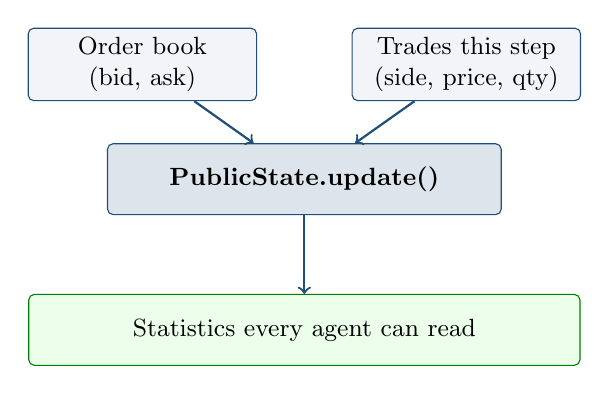
\begin{tikzpicture}[node distance=1.2cm, every node/.style={font=\small},
  box/.style={draw=accent, rounded corners=2pt, fill=accent!6, minimum height=0.9cm,
              minimum width=2.9cm, align=center}]
  \node[box] (book) {Order book\\ (bid, ask)};
  \node[box, right=of book] (trades) {Trades this step\\ (side, price, qty)};
  \node[box, below=1.0cm of $(book)!0.5!(trades)$, minimum width=5cm, fill=accent!15] (ps)
        {\textbf{PublicState.update()}};
  \node[box, below=1.0cm of ps, minimum width=7cm, fill=green!8, draw=green!50!black]
        (out) {Statistics every agent can read};
  \draw[->, thick, accent] (book) -- (ps);
  \draw[->, thick, accent] (trades) -- (ps);
  \draw[->, thick, accent] (ps) -- (out);
\end{tikzpicture}
\end{center}

The variables fall into six families:

\begin{center}
\renewcommand{\arraystretch}{1.25}
\begin{tabular}{@{}L{3.6cm}L{10.6cm}@{}}
\toprule
\textbf{Family} & \textbf{Question it answers}\\
\midrule
Price and book    & Where is the market right now, and how expensive is it to trade?\\
Moving averages   & What is the ``typical'' recent price level?\\
Volatility        & How jumpy is the price?\\
Volume            & How much is being traded?\\
Momentum          & Is the price trending up or down?\\
Order-flow balance& Are buyers or sellers pushing harder?\\
Attention         & Is the market unusually active right now?\\
\bottomrule
\end{tabular}
\end{center}

%==================================================================================================
\section{A key tool: the exponential moving average}
\label{sec:ewma}

Most variables below use an \textbf{exponentially weighted moving average} (EWMA, or EMA). It is a
running average that gives more weight to recent data and slowly forgets the past. The update is a
single line:
\begin{equation}
  \text{avg}_{\text{new}} \;=\; \text{avg}_{\text{old}} + \alpha\,\bigl(x_{\text{new}} - \text{avg}_{\text{old}}\bigr),
  \qquad \alpha = \frac{2}{\text{span}+1}.
  \label{eq:ewma}
\end{equation}

\begin{intuition}
Think of the average as a thermometer reading that moves a fraction $\alpha$ of the way toward each
new observation. A \emph{short span} gives a big $\alpha$: the average reacts quickly. A \emph{long
span} gives a small $\alpha$: the average is smooth and slow.
\end{intuition}

\begin{example}
Span $=9$ gives $\alpha = 0.2$. If the average is $100$ and the new value is $110$, the average
moves to $100 + 0.2\cdot 10 = 102$.
\end{example}

\begin{whyuse}
It needs only \emph{one stored number} per statistic (no history list), so each update costs the same
tiny amount of work however long the simulation runs.
\end{whyuse}

The simulator uses two spans, set in \code{PublicStateConfig}: a \textbf{fast} one (default
10 steps) and a \textbf{slow} one (default 100 steps). Comparing the two tells us whether
\emph{now} looks different from \emph{normal}. This idea comes back again and again below.

%==================================================================================================
\section{Price and book variables}

\subsection{\code{best\_bid}, \code{best\_ask}, \code{spread}}
The best bid and best ask are read directly from the book. The spread is their gap:
\[
  \text{spread} = \text{best\_ask} - \text{best\_bid}.
\]
\begin{whyuse}
The spread is the immediate cost of trading: buying at the ask and selling at the bid loses the
spread. Market makers use it to decide where to quote, and execution strategies use it to judge how
expensive it is to be impatient.
\end{whyuse}

\subsection{\code{mid}}
The \textbf{mid-price} is the midpoint of the best quotes:
\[
  \text{mid} = \frac{\text{best\_bid} + \text{best\_ask}}{2}.
\]
If one side of the book is empty, it falls back to the \code{last} trade price, and if there has been
no trade, it keeps the previous mid.

\begin{whyuse}
There is no single ``true'' price, but the mid is a smooth, fair-looking reference that does not
jump around every time a trade bounces between bid and ask. Every statistic below is built on it.
\end{whyuse}

\subsection{\code{last}}
The price of the most recent trade (or \code{None} if nothing has traded yet). It is mostly used as
the fallback for the mid described above.

%==================================================================================================
\section{Moving averages of price}

\subsection{\code{ma\_fast} and \code{ma\_slow}}
Two EWMAs (Eq.~\ref{eq:ewma}) of the mid-price, one with the fast span and one with the slow span.

\begin{intuition}
\code{ma\_fast} hugs the current price. \code{ma\_slow} is a lazy long-term anchor. When the two
differ, the price has recently moved away from its long-run level.
\end{intuition}

\begin{whyuse}
They give agents a cheap estimate of ``where the price usually is''. For example, a mean-reverting
speculator may buy when the price is well below the slow average.
\end{whyuse}

%==================================================================================================
\section{Volatility}

\subsection{\code{var\_fast} and \code{var\_slow}}
Volatility measures how much the price jumps around. At each step we compute the mid-price change
$\Delta = \text{mid}_t - \text{mid}_{t-1}$ and take an EWMA of its square:
\[
  \text{var} \leftarrow \text{var} + \alpha\bigl(\Delta^2 - \text{var}\bigr).
\]
The unit is \emph{ticks$^2$ per step} (a tick is the smallest allowed price increment). Both start
at $1$ to avoid dividing by zero later.

\begin{example}
If the price moves $+2,\,-2,\,+2,\,-2$ ticks, $\Delta^2=4$ every time, so the variance tends to $4$.
A quiet market with moves of $0$ or $\pm1$ has variance below $1$.
\end{example}

\begin{whyuse}
Volatility is the market's mood: wide quotes and cautious behaviour in turbulent times, tight quotes
in calm times. The \emph{ratio} of the fast to the slow value flags sudden regime changes
(Section~\ref{sec:attention}).
\end{whyuse}

%==================================================================================================
\section{Volume}

\subsection{\code{step\_volume}}
The total aggressive volume traded in the current step: $\text{buy\_volume} + \text{sell\_volume}$.

\subsection{\code{volume\_fast} and \code{volume\_slow}}
EWMAs of \code{step\_volume} at the two horizons.

\begin{whyuse}
Volume shows how much participation there is. A burst of volume with \code{volume\_fast} far above
\code{volume\_slow} means something is happening, and that is the second ingredient of the attention
multiplier.
\end{whyuse}

%==================================================================================================
\section{Momentum}

\subsection{\code{momentum}}
\code{momentum} is a \emph{list}, one entry for each (fast, slow) pair in \code{lookbacks}. The
defaults are $(5,30)$, $(10,60)$ and $(20,120)$. For each pair we keep two EWMAs of the mid-price with
those spans, and define
\[
  \text{momentum}_k = \text{EMA}_{\text{fast},k}(\text{mid}) - \text{EMA}_{\text{slow},k}(\text{mid}).
\]

\begin{intuition}
If the price has been rising, the quick average sits above the slow one, so momentum is
\textbf{positive}. If it has been falling, momentum is \textbf{negative}. A value near zero means no
clear trend. Using three pairs gives a short-, medium- and long-term view of the trend.
\end{intuition}

\begin{whyuse}
Trend-following traders buy when momentum is positive and sell when it is negative. Because many
agents react to it, it also makes the simulated market behave more like real ones, where trends can
feed on themselves.
\end{whyuse}

%==================================================================================================
\section{Signed aggressive flow}

\subsection{\code{buy\_flow}, \code{sell\_flow}}
Rolling totals of aggressive buy volume and aggressive sell volume over the last \code{flow\_window}
steps (default 20). Internally, a circular buffer stores the last 20 values; when a new step arrives
it overwrites the oldest one and the running totals are adjusted by (new $-$ old). That makes each
update $O(1)$.

\subsection{\code{imbalance}}
\[
  \text{imbalance} = \frac{\text{buy\_flow} - \text{sell\_flow}}{\text{buy\_flow} + \text{sell\_flow}}
  \;\in\;[-1,\,1],
\]
and $0$ if nothing has traded.

\begin{example}
$\text{imbalance}=+1$: only buyers were aggressive. $0$: perfectly balanced. $-0.5$: sellers did
three times as much aggressive volume as buyers.
\end{example}

\begin{whyuse}
Random trading is roughly balanced. A big institution splitting a huge order into many small ones
(a \emph{metaorder}) pushes the flow persistently one way. This variable is the raw footprint that
detectors and liquidity providers look at to spot such activity, which is exactly what the research
project studies. The class itself only \emph{computes} the numbers; interpreting them is left to
\code{order\_book.detectors}.
\end{whyuse}

\subsection{\code{step\_trades}}
The list of anonymous aggressive trades of the current step, each as
\code{(side, price, quantity)}. Trader identities are deliberately not included.

\begin{whyuse}
It gives agents and detectors trade-by-trade detail while preserving anonymity, as on a real exchange
tape.
\end{whyuse}

%==================================================================================================
\section{The attention multiplier}
\label{sec:attention}

\subsection{\code{attention}}
This one combines volatility and volume into a single activity dial. First compare ``now'' with
``normal'':
\[
  r_{\text{vol}} = \sqrt{\frac{\text{var\_fast}}{\text{var\_slow}}},
  \qquad
  r_{\text{volume}} = \frac{\text{volume\_fast}}{\text{volume\_slow}}.
\]
Each ratio is $1$ when things are normal, above $1$ when the market is busier than usual, and below
$1$ when it is quieter. Then
\[
  \text{attention} = \operatorname{clamp}\!\Bigl(1 + \tfrac12(r_{\text{vol}}-1) + \tfrac12(r_{\text{volume}}-1),\; 0.5,\; 3\Bigr).
\]

\begin{example}
Volatility is 50\% above normal ($r_{\text{vol}}=1.5$) and volume is double ($r_{\text{volume}}=2$):
$1 + 0.25 + 0.5 = 1.75$. Agents are $1.75\times$ as active as usual. A very quiet market bottoms out
at $0.5$, and a frenzy is capped at $3$.
\end{example}

\begin{whyuse}
Real markets show \textbf{activity clustering}: busy periods attract more activity, and calm periods
stay calm. Agents multiply their order-arrival rates by \code{attention}, so the simulator reproduces
that behaviour. The clamp keeps it from exploding or dying out.
\end{whyuse}

\subsection{\code{warmed\_up}}
The slow averages need time to become meaningful. Early on they are still close to their initial
values, so the ratios above would be nonsense. \code{warmed\_up} turns \code{True} once
$n\cdot\alpha_{\text{slow}}>1$, i.e.\ after roughly one slow span of data. Until then, \code{attention}
stays at $1$.

%==================================================================================================
\section{Bookkeeping}

\begin{description}[leftmargin=3.2cm, style=nextline]
  \item[\code{step\_count}] The number of updates so far.
\end{description}

%==================================================================================================
\section{Cheat sheet}

\renewcommand{\arraystretch}{1.3}
\begin{center}
\small
\begin{tabular}{@{}L{3.2cm}L{6.4cm}L{5.4cm}@{}}
\toprule
\textbf{Variable} & \textbf{What it is} & \textbf{Typically used for}\\
\midrule
\code{best\_bid / best\_ask} & Best buy and sell offers & Quoting, trading cost\\
\code{spread} & Ask minus bid & Cost of trading now\\
\code{mid} & Midpoint of the quotes & Reference price\\
\code{last} & Last trade price & Fallback price\\
\code{ma\_fast / ma\_slow} & Smoothed price, short and long & Mean-reversion signals\\
\code{var\_fast / var\_slow} & Smoothed squared price change & Volatility regime\\
\code{step\_volume} & Volume traded this step & Activity measure\\
\code{volume\_fast / slow} & Smoothed volume & Activity regime\\
\code{momentum[k]} & Fast EMA $-$ slow EMA, per pair & Trend following\\
\code{buy\_flow / sell\_flow} & Rolling aggressive volume per side & Pressure measurement\\
\code{imbalance} & Normalised buy/sell difference in $[-1,1]$ & Spotting one-sided execution\\
\code{step\_trades} & Anonymous trades this step & Tape-level detail\\
\code{attention} & Activity multiplier in $[0.5,3]$ & Activity clustering\\
\code{warmed\_up} & Slow averages are reliable & Guarding ratios\\
\code{step\_count} & Number of updates & Bookkeeping\\
\bottomrule
\end{tabular}
\end{center}

\section{Default parameters}

All parameters live in \code{PublicStateConfig} (\code{order\_book/config.py}).

\begin{center}
\renewcommand{\arraystretch}{1.25}
\begin{tabular}{@{}L{3.2cm}L{3.2cm}L{7.6cm}@{}}
\toprule
\textbf{Parameter} & \textbf{Default} & \textbf{Meaning}\\
\midrule
\code{fast}        & 10 & EWMA span of the fast price, variance and volume statistics\\
\code{slow}        & 100 & EWMA span of the slow statistics\\
\code{lookbacks}   & (5,30), (10,60), (20,120) & (fast, slow) span pairs for momentum\\
\code{flow\_window}& 20 & Steps kept in the rolling signed-flow window\\
\bottomrule
\end{tabular}
\end{center}

\end{document}
